
\section{Takeaways: Experimental Findings Verification and Explanation}
\label{sec:takeaways}

We apply our proposed formulation to validate and provide a theoretical explanation for numerous existing experimental findings regarding the training dynamics of language models. These key insights also guide researchers in selecting critical LRS before initiating model training. An interesting summary is that
\begin{quotation}
{\color{magenta}\textit{The art of learning rate schedule lies in the delicate balancing act between forward area and annealing area.}}
\end{quotation}

\subsection{\color{cyan} It verifies and explains why loss drops more sharply when LR anneals.}
\label{apx:takeaway-sharpdrop}
Our equation helps researchers understand why loss values drop more sharply when LR anneals. This phenomenon has been widely observed in many previous studies.
Without loss of generality, consider the fitted equation from Fig.~\ref{fig:fit}.
We analyze how the $S_1$-item ($A\cdot S_1^{-\alpha}$) and the negative $S_2$-item ($-C\cdot S_2$) impact the loss values (notated as ``$\Delta$Loss'') obtained across a WSD scheduler (see Fig.~\ref{fig:phe-sharp}). It can be seen that in the annealing stage, the negative $S_2$-item has a much more significant impact on the overall loss than the $S_1$-item. Therefore, the loss drops more sharply compared to the stage with constant LR.
In conclusion, LR annealing increases the annealing area, which further leads to a drastic decrease for the validation loss.



\begin{figure}[tbp]
\centering
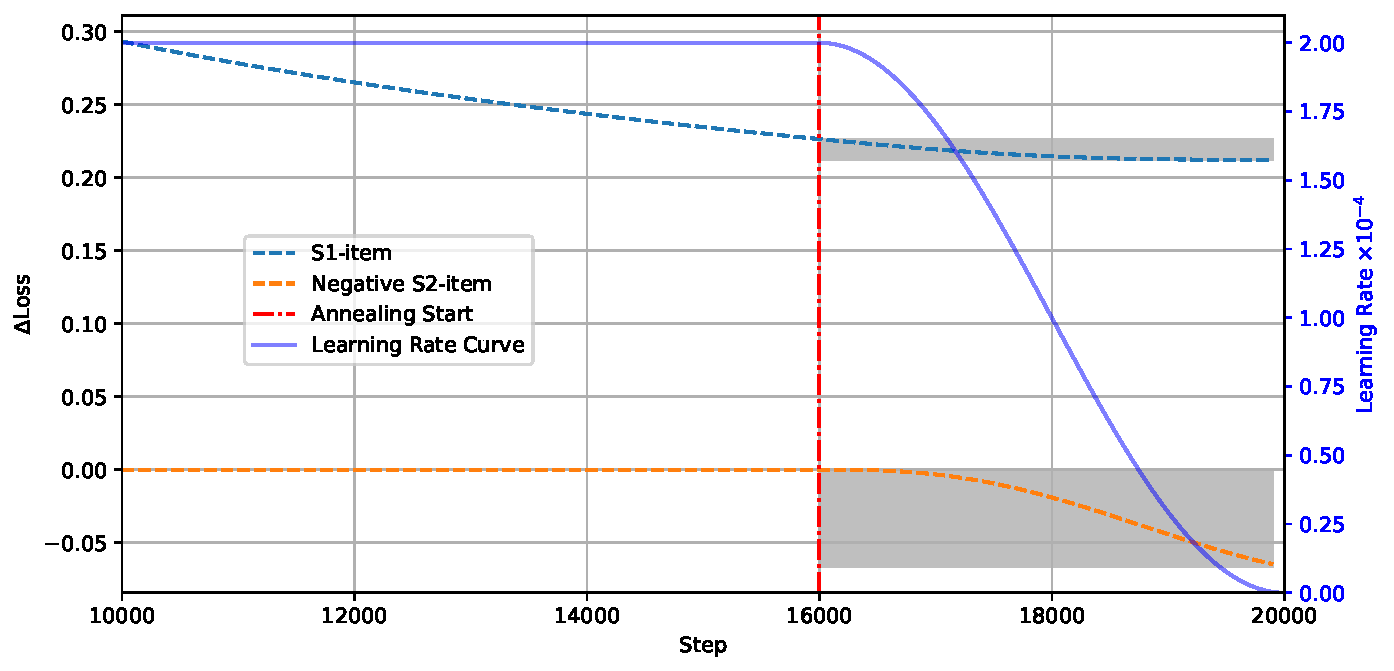
\includegraphics[width=0.7\textwidth]{images/draw_phe/wide-1.pdf}
\caption{How S1-item and negative $S_2$-item changes in a WSD LRS. The upper and lower shaded area indicate the loss drop brought by $S_1$ and $S_2$, respectively, in the annealing stage.}
\label{fig:phe-sharp}
\end{figure}



\subsection{\color{cyan} Determining cosine cycle length and minimum LR in cosine LRS.}
Many papers have found that in LLM pre-training using cosine LRS, setting the cosine cycle length $T$ as the total steps $S$, and setting min LR as nearly 0 (rather than 10\% max LR) can lead to the optimal loss~\citep{hoffmann2022training,hu2024minicpm,hägele2024scaling,parmar2024reuse}. 
% Actually, the settings above have been a factual standard in LLM pre-training using cosine LRS.
We theoretically validate this observation using our equation in Fig.~\ref{fig:phe-cosine}. The predicted loss curve with $T=S$ and a minimum LR of 0 indeed achieves the optimal loss in the final step.
Moreover, our equation gives a quite intuitive explanation: setting $T>S$ leads to incomplete annealing, while $T<S$ leads to a small forward area $S_1$ due to early annealing. Thus, the optimal configuration is to set $T$ equal to $S$. Also, setting the minimum LR to $0$ maximizes the annealing amount, thereby increasing the annealing area $S_2$, which facilitates lower final loss.


\begin{figure}[htbp]
    \centering
    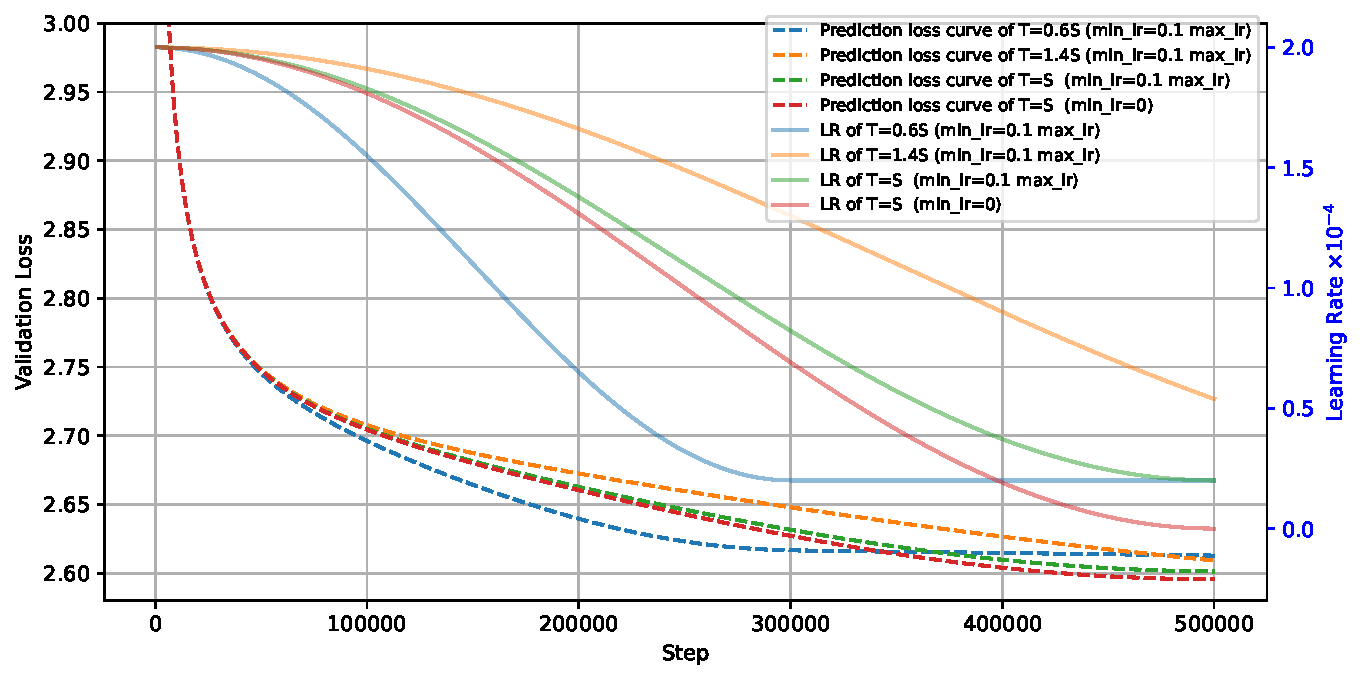
\includegraphics[width=0.7\linewidth]{images/draw_phe/wide-3-2.pdf}
    \caption{Predicted loss curves of different cycle length $T$ and min LR in cosine LRS. The results well align with previous studies.}
\label{fig:phe-cosine}
\end{figure}



\subsection{\color{cyan} It verifies and explains the phenomenon, where constant LRS gets a lower loss than cosine LRS if setting small total steps, and vice versa.}
\label{apx:takeaway-constant-cosine}
\begin{figure}[ht]
    \centering
    \begin{subfigure}[b]{0.32\textwidth}
        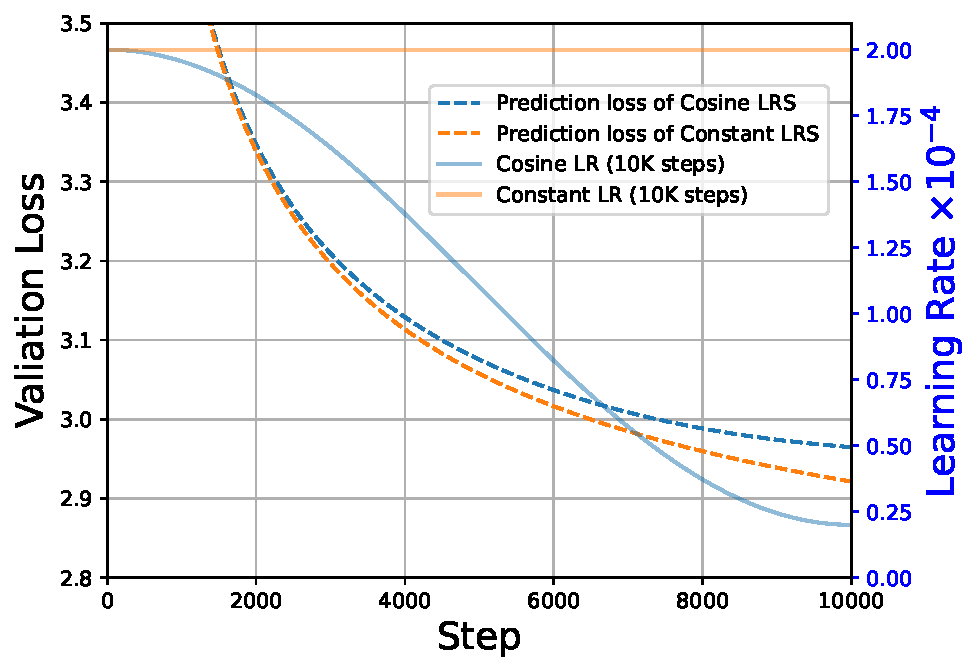
\includegraphics[width=\textwidth]{images/draw_phe/4-1.pdf}
        \caption{The predicted loss curve of 10K total steps.}
    \end{subfigure}
    \hfill
    \begin{subfigure}[b]{0.32\textwidth}
        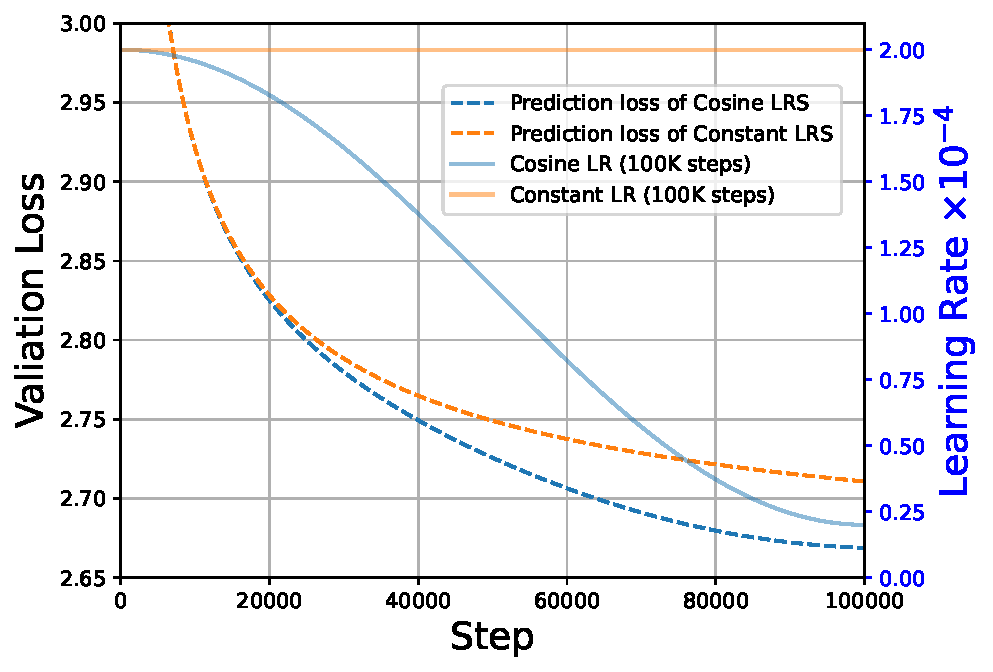
\includegraphics[width=\textwidth]{images/draw_phe/4-2.pdf}
        \caption{The predicted loss curve of 100K total steps.}
    \end{subfigure}
    \hfill
    \begin{subfigure}[b]{0.288\textwidth}
        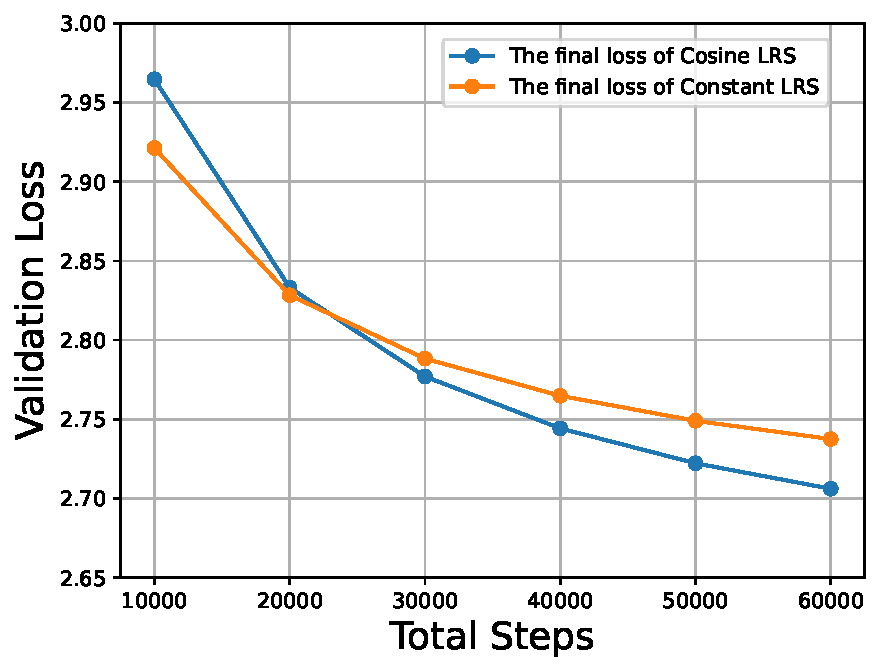
\includegraphics[width=\textwidth]{images/draw_phe/4-3.pdf}
        \caption{The predicted final loss of different total steps.}
        \label{fig:phe-constant-cosine-final}
    \end{subfigure}
    \caption{Predicted loss curves and final losses for the constant and cosine LRS.}
\label{fig:phe-constant-cosine}
\end{figure}

In our experiments shown in Fig.~\ref{fig:fit}, we observe that the constant LRS can sometimes yield lower final loss values than the cosine LRS.
To validate this phenomenon, we use our equation to predict the loss curve of a constant and cosine LRS for 10K and 100K total steps in Fig.~\ref{fig:phe-constant-cosine}. It can be seen that with more training steps, the cosine LRS outperform the constant LRS, while with less training steps, the constant LRS is better.
Moreover, Fig.~\ref{fig:phe-constant-cosine-final} shows the predicted final loss of different total steps using constant and cosine LRS. It further convincingly suggests that constant LRS indeed gets a lower loss if setting small total steps, but the scaling slope is smaller than cosine LRS's, resulting in higher loss in more steps.

We can further analyze this phenomenon by taking the derivative of $S_1$ and $S_2$ of Eq.~\ref{eq:scaling}. Specifically, $|\frac{\partial L}{\partial S_1}| = \alpha A \cdot S_1^{-\alpha-1}$ is a power-law decreasing function while $|\frac{\partial L}{\partial S_2}| = C$ is a constant.
When the training step $s$ is small, $|\frac{\partial L}{\partial S_1}|$ is larger than $|\frac{\partial L}{\partial S_2}|$ since we have a small $S_1$. Therefore $S_1$ plays a dominant role over $S_2$. In this case, increasing $S_1$ by maintaining a large LR, i.e. using a constant LRS rather than a cosine LRS, leads to more sharply decrease of the loss value.

When the training step $s$ is large,
$|\frac{\partial L}{\partial S_1}|$ becomes smaller than $|\frac{\partial L}{\partial S_2}|$. Therefore, $S_2$ plays a dominant role over $S_1$. In this case, increasing $S_1$ does not contribute much for decreasing the loss. It is time to start LR annealing to increase $S_2$. 
Interestingly, this formulation aligns with the idea of WSD LRS~\citep{hu2024minicpm}: 
In the early stages, the neural network is exploring globally and it is a suitable time to use a larger LR; In the later stages, the neural network is exploring locally and it is a suitable time to use a smaller LR.
We will delve further into WSD LRS in the following subsections.

\subsection{\color{cyan} It verifies and explains WSD and multi-step cosine LRS have matched or even lower loss than cosine LRS.}
\begin{figure}[htbp]
    \centering
    \begin{subfigure}[b]{0.48\textwidth}
        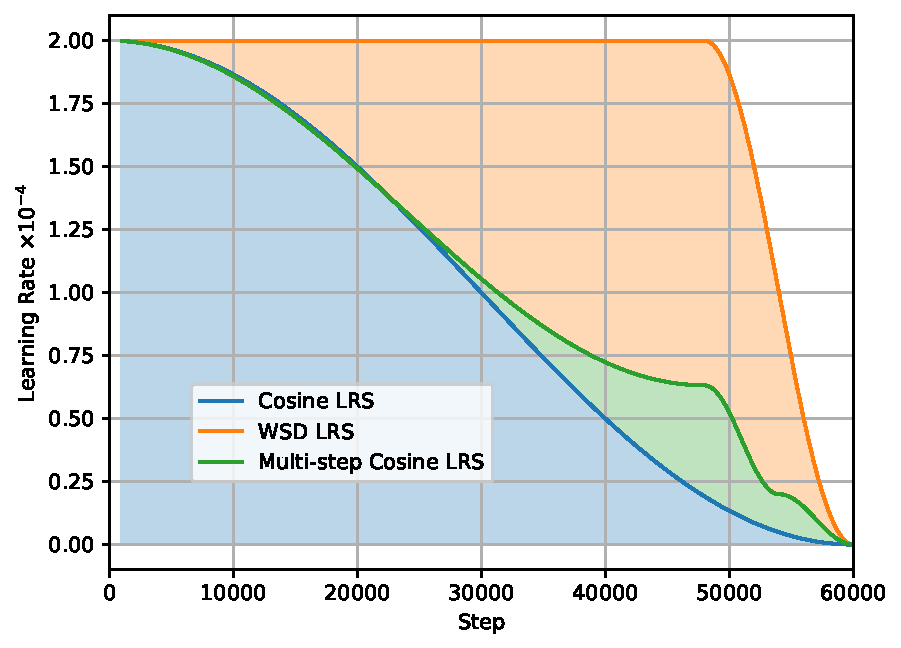
\includegraphics[width=\textwidth]{images/draw_phe/2.pdf}
        \caption{Learning rate curves of three types of LRS.}
    \end{subfigure}
    \hfill
    \centering
    \begin{subfigure}[b]{0.48\textwidth}
        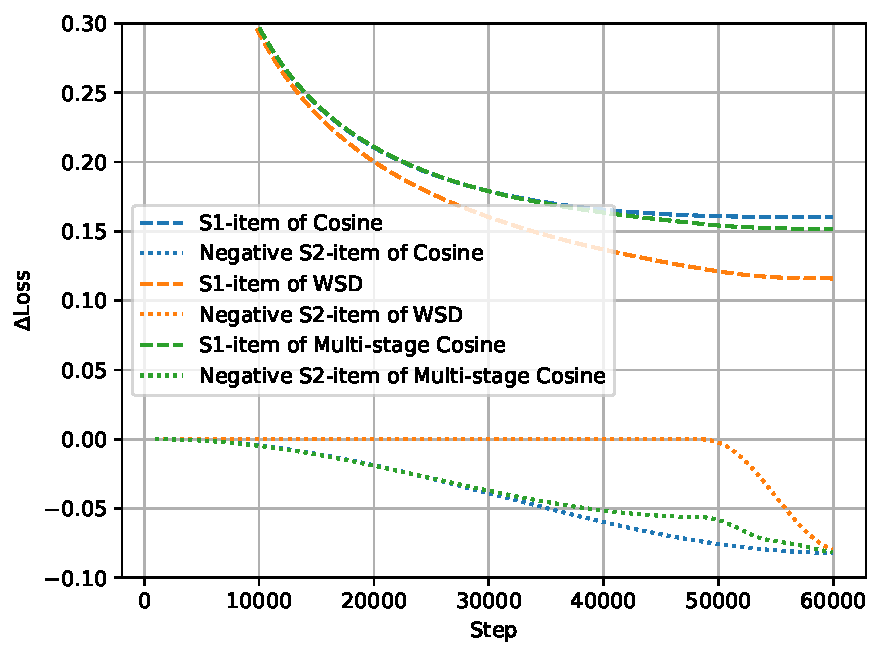
\includegraphics[width=\textwidth]{images/draw_phe/2-2.pdf}
        \caption{$S_1$-item and negative $S_2$-item of different LRS.}
    \end{subfigure}
    \caption{The comparison between $S_1$-item and negative $S_2$-item in different LRS.}
\label{fig:phe-match}
\end{figure}

Recent studies have shown that WSD LRS~\citep{hu2024minicpm} and multi-step cosine LRS~\citep{deepseek-ai2024deepseek} result in lower loss compared to the traditional cosine LRS. 
Our experiments also support this finding (refer to the ground-truth loss in Fig.~\ref{fig:prediction-cosine},~\ref{fig:prediction-multi-cosine},~\ref{fig:prediction-wsd}). 
We validate and elucidate this finding using our proposed equation. Fig.~\ref{fig:phe-match} shows the learning rate curve (left) and the predicted loss drop (right) for different LRS.
The results suggest that for WSD and multi-step cosine LRS, the negative $S_2$-item ($-C\cdot S_2$) is slightly larger than that of the cosine LRS, whereas the $S_1$-item ($A\cdot S_1^{-\alpha}$) is significantly lower.
Specifically, both the WSD LRS and multi-step cosine LRS unintentionally employ strategies that marginally reduces $S_2$ but substantially increases $S_1$, leading to an overall decrease in validation loss.


\subsection{\color{cyan} Determining Optimal Annealing Ratio of WSD LRS.}
In the case of WSD LRS, it is crucial to ascertain the optimal annealing ratio for training steps. 
~\citet{hägele2024scaling} found that there is an optimal annealing ratio for WSD LRS, i.e. both excessively high or low annealing ratios lead to sub-optimal model performance. 
This phenomenon can be further elucidated through our proposed equation. 
Specifically, a high annealing ratio results in a significant reduction of the forward area $S_1$ while a low annealing ratio leads a diminished annealing area $S_2$. 
Our scaling law equation describes the trade-off between the forward area $S_1$ and the annealing area $S_2$ about the annealing ratio.

Fig.~\ref{fig:phe-match:1} depicts the final loss predicted by our equation for various annealing ratios and total training steps. 
The predictions form parabola-like curves, and align well with the actual experimental results reported in previous studies.
This suggests that a moderate annealing ratio, typically around 10\% to 20\%, is optimal, as it balances $S_1$ and $S_2$ to maximize their combined effect, thereby minimizing the overall validation loss.
Moreover, our equation can directly predict the optimal annealing ratio for different total steps without large-scale experiments, which saves a lot of resources. 


\begin{figure}[tbp]
    \centering
    \begin{subfigure}[b]{0.48\textwidth}
        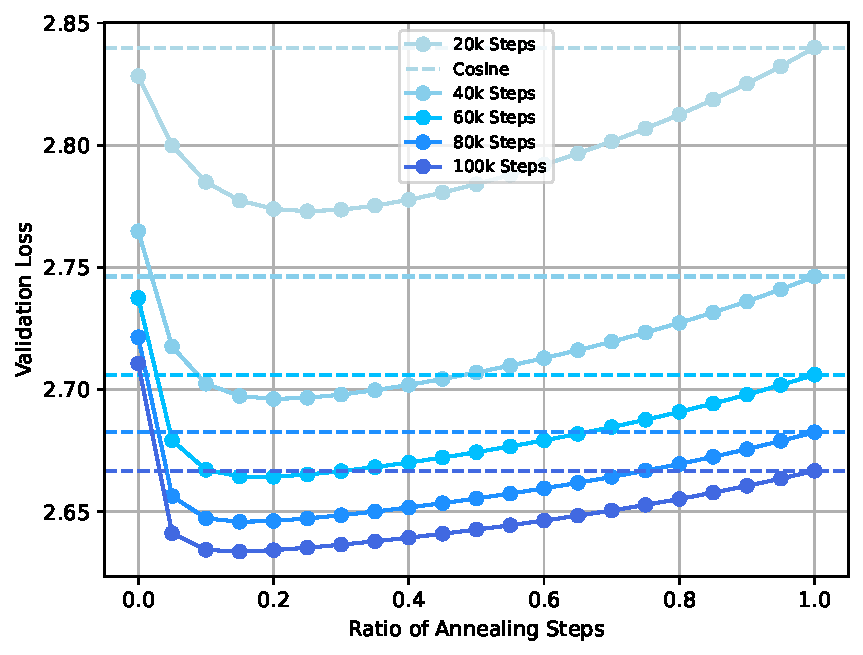
\includegraphics[width=\textwidth]{images/wsd_ratio.pdf}
        \caption{The relationship between the predicted final loss and the ratio of annealing steps under the condition of different total steps.}
    \end{subfigure}
    \hfill
    \begin{subfigure}[b]{0.48\textwidth}
        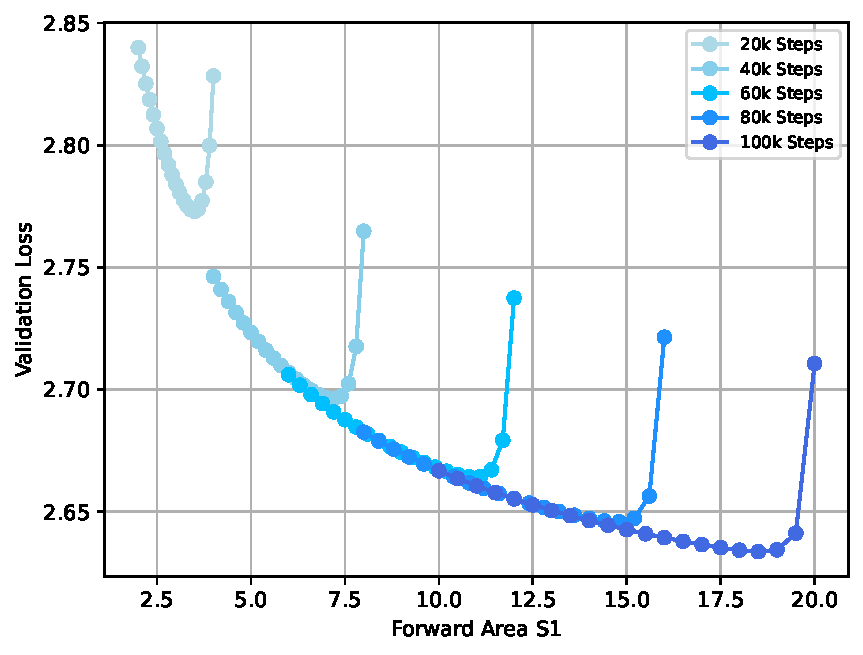
\includegraphics[width=\textwidth]{images/s1_loss.pdf}
        \caption{The relationship between predicted final loss and the forward area $S_1$ of different total steps. Different points denote different annealing ratios.}
    \end{subfigure}
    \caption{Illustration of the predicted loss in relation to the ratio of annealing steps and the forward area in WSD LRS (cosine annealing), presenting parabola-like curves, with a distinct optimal loss.}
\label{fig:phe-match:1}
\end{figure}



\subsection{\color{cyan} Determining the optimal annealing function in WSD LRS.}
\label{apx:takeaway-anneal-func}
\begin{figure}[tbp]
    \centering
    \begin{subfigure}[b]{0.48\textwidth}
        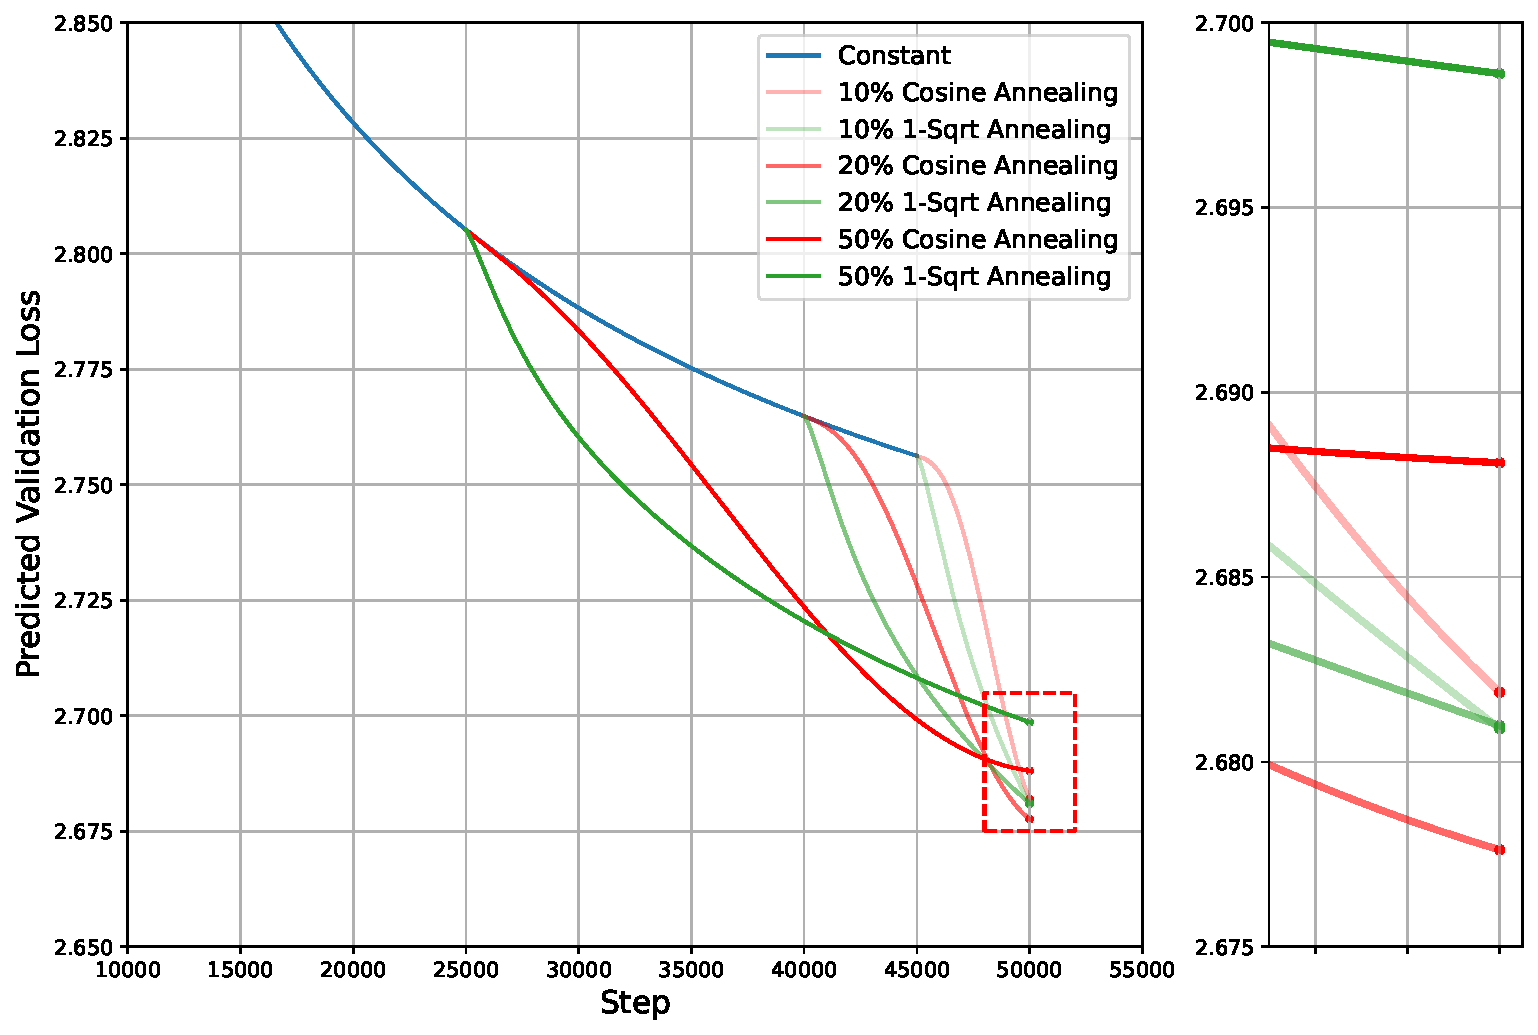
\includegraphics[width=\textwidth]{images/plot_newxy/cosine_sqrt_1.pdf}
        \caption{The \textbf{predicted} loss curve of cosine and 1-sqrt annealing method of different annealing ratio.}
        \label{fig:phe-diff-anneal-predict}
    \end{subfigure}
    \hfill
    \begin{subfigure}[b]{0.48\textwidth}
        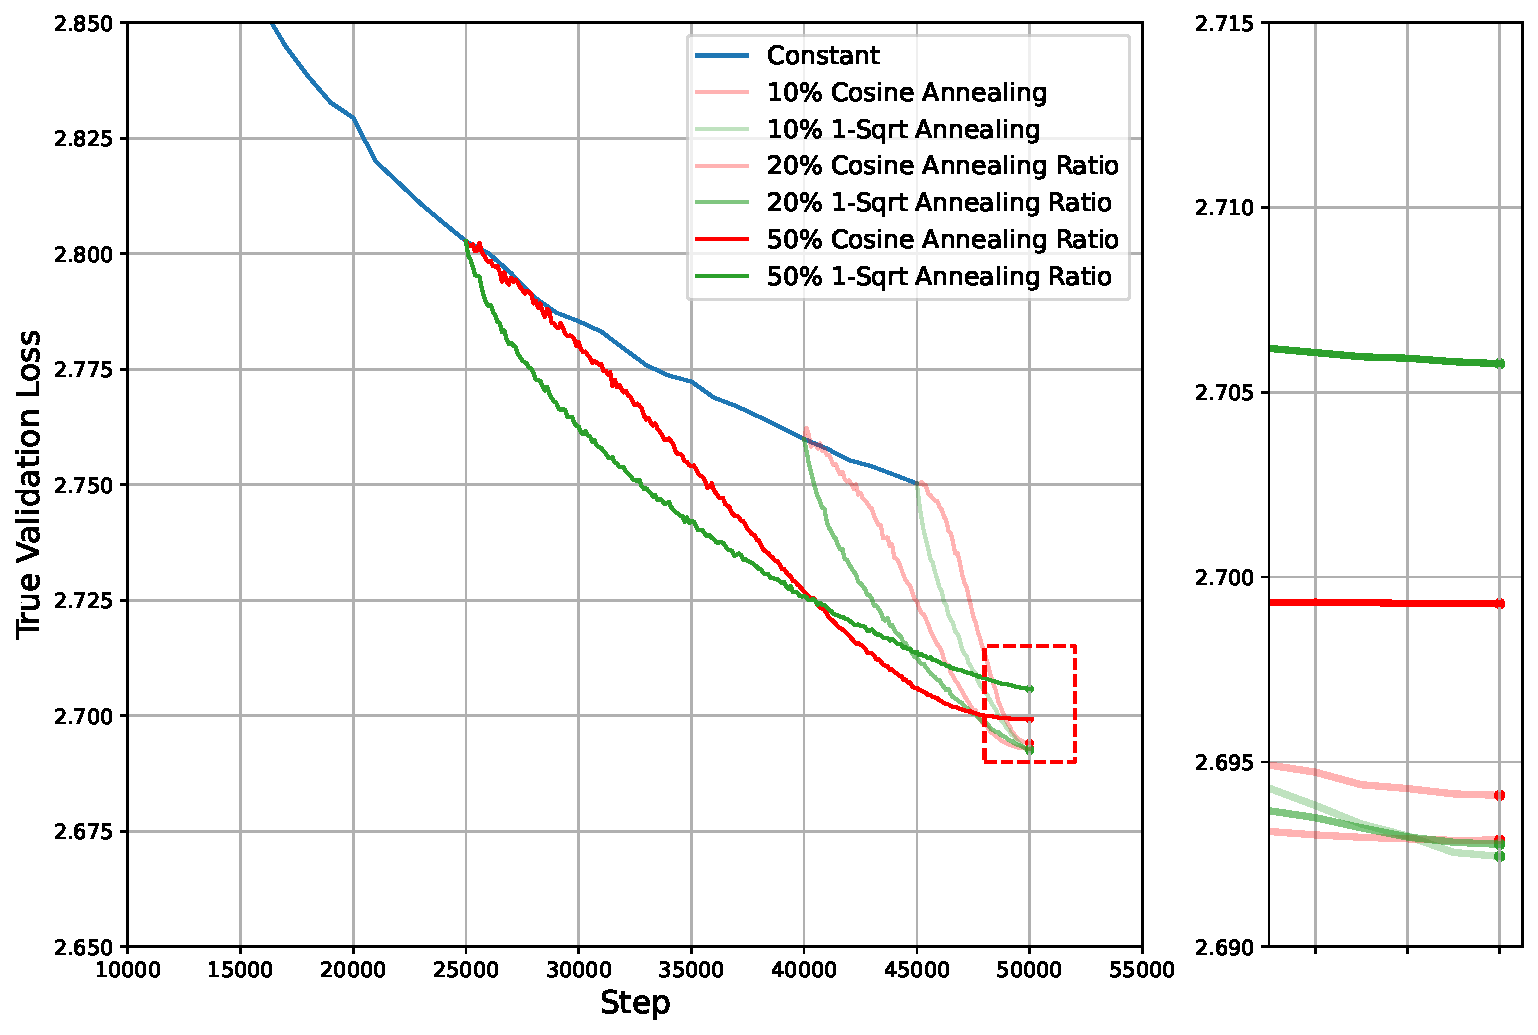
\includegraphics[width=\textwidth]{images/plot_newxy/cosine_sqrt_2.pdf}
        \caption{The \textbf{true} loss curve of different annealing ratios with cosine and 1-sqrt annealing methods.}
        \label{fig:phe-diff-anneal-true}
    \end{subfigure}
    \caption{The predicted (left) and true loss (right) of cosine and 1-sqrt annealing method at different annealing ratios. Experimental results (right), aligned with our prediction (left), refute the claim ``the order and results of different annealing hold across settings''~\citep{hägele2024scaling}.}
\label{fig:phe-diff-anneal}
\end{figure}

For the WSD LRS, the selection of the annealing function is another important factor for obtaining further lower loss values. \citet{hägele2024scaling} conclude that the 1-sqrt annealing (see Appendix~\ref{apx:1-sqrt} for the detailed formula) yields lower final losses compared to the other annealing methods (e.g. cosine). 
They claim that this conclusion is true across different annealing ratios.

However, our equation suggests different results (see Fig.~\ref{fig:phe-diff-anneal-predict}). The 1-sqrt annealing approach does get a lower loss than the cosine annealing approach when using small annealing ratios (e.g. 10\%), but it performs much worse than the cosine annealing approach when using 50\% annealing ratio.

To verify our prediction, we conduct experiments by training models using different annealing methods and ratios within 50K total steps. As illustrated in Fig.~\ref{fig:phe-diff-anneal-true}, at a 10\% annealing ratio, the 1-sqrt annealing method obtains lower final losses compared to the cosine annealing method, whereas at a 50\% annealing ratio, the cosine annealing method obtains a lower final loss compared to the 1-sqrt annealing method. The experimental results align quite well with our prediction, which also overturns some of the claims made by previous works. We conclude that the optimal annealing function in WSD LRS depends on the annealing ratio.

Our scaling law equation provides an explanatory framework for these empirical observations. We draw the LR curves associated with the 1-sqrt and cosine annealing approaches in Appendix~\ref{apx:1-sqrt}.
When using an small annealing ratio, the forward area \(S_1\) of the cosine annealing method is slightly larger than that of the 1-sqrt annealing method, while the annealing area \(S_2\) of the 1-sqrt method plays a more dominate role in decreasing the final loss. As the annealing ratio increases, the difference of $S_1$ between two annealing methods becomes larger and larger. Therefore the forward area \(S_1\) gradually takes the dominate role. The delicate balance between $S_1$ and $S_2$ breaks at 50\% annealing ratio, resulting in a lower final loss for the cosine annealing function.

The above analysis underscores the importance of carefully selecting the annealing strategy for the WSD LRS to optimize model training outcomes. Our equation can help predict a better annealing function without experiments, which saves a lot of resources. 

\subsection{\color{cyan} It verifies and explains that in continual pre-training, a higher max learning rate during re-warmup leads to a higher initial peak in the loss, followed by a more rapid decrease.}
\label{apx:takeaway-cpt-peaklr}

In continual pre-training (CPT) settings, the LRS typically involves re-warmup to a new max LR at the start of training. 
Through numerous experiments,~\citet{gupta2023continualpretraininglargelanguage} concludes that a higher max LR during re-warmup results in a higher initial peak loss, followed by a more rapid decrease. 

According to our scaling law formulation~\footnote{Strictly speaking, continual pre-training process often include LR re-warmup as well as data distribution shift. Here we primarily research on the setting that there is no distribution shift between two training stages. The conclusions transfer across most cases because the loss change brought by LR re-warmup is significantly larger than the loss change brought by data distribution shift~\citep{gupta2023continualpretraininglargelanguage,simple-scalable-cpt2024}.}, in the LR re-warmup process, the annealing area $S_{2}$ will reduce to a negative value ($S_2<0$) and thus the validation loss increases. A higher max LR in re-warmup lead to a lower annealing area $S_{2}$, and thus there would be a higher peak loss. 
Moreover, a higher max LR also leads to a faster growth of the forward area $S_{1}$ after re-warmup. We use the fitted equation to predict the continual pre-training process with different max LR as shown in Fig.~\ref{fig:phe-match-cpt-lr}. The predicted loss curves reproduce a quite similar phenomenon with previous works~\citep{gupta2023continualpretraininglargelanguage}. 

There is a more profound strategy using our equation in CPT. As shown in Fig.~\ref{fig:phe-match-cpt-lr}, after the total steps of CPT is determined, we can apply our equation to predict a better max LR and scheduler to get the lowest final loss without experiments, which saves a lot of resources.

\subsection{\color{cyan} It verifies and explains that in continual pre-training, the steps of re-warmup have little impact on the final loss.}
\label{apx:takeaway-cpt-step}

Meanwhile, how many steps to re-warmup is another important issue in the continual pre-training.
~\citet{gupta2023continualpretraininglargelanguage} find that longer re-warmup steps smooth the transition of loss curve but the number of re-warmup steps does not significantly influence the final validation loss. 
We use the fitted equation to predict the continual pre-training dynamics with different re-warmup steps. The results, shown in Fig.~\ref{fig:phe-match-cpt-step}, present a good alignment with previous observations~\citep{gupta2023continualpretraininglargelanguage}. 

Based on our theory, given a fixed max LR, longer re-warmup steps lead to a slower decreases of the annealing area, resulting in a smoother raise in the loss curve. However, both the final values of the forward area ($S_1$) and the annealing area ($S_2$) remain relatively stable across different re-warmup steps. The annealing area ($S_2$) corresponding to different re-warmup steps are very close since the max and min LR remain the same. 
Besides, although different re-warmup steps lead to temporary distinct loss fluctuations, re-warmup only accounts for a small portion of the whole training process. Thus, the forward area $S_1$ is also close across different re-warmup steps, resulting in the close overall loss across different steps of re-warmup.

\begin{figure}[tbp]
    \centering
    \begin{subfigure}[b]{0.48\textwidth}
        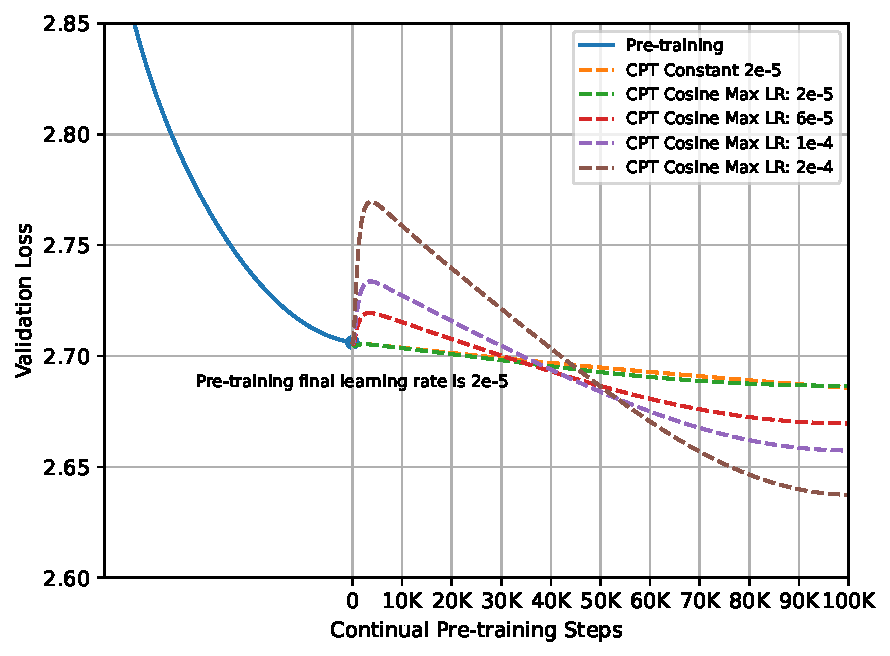
\includegraphics[width=\textwidth]{images/max_lr.pdf}
        \caption{The predicted validation loss with different re-warmup max LR in the continual pre-training process. All the re-warmup steps are 500 steps. }
        \label{fig:phe-match-cpt-lr}
    \end{subfigure}
    \hfill
    \begin{subfigure}[b]{0.48\textwidth}
        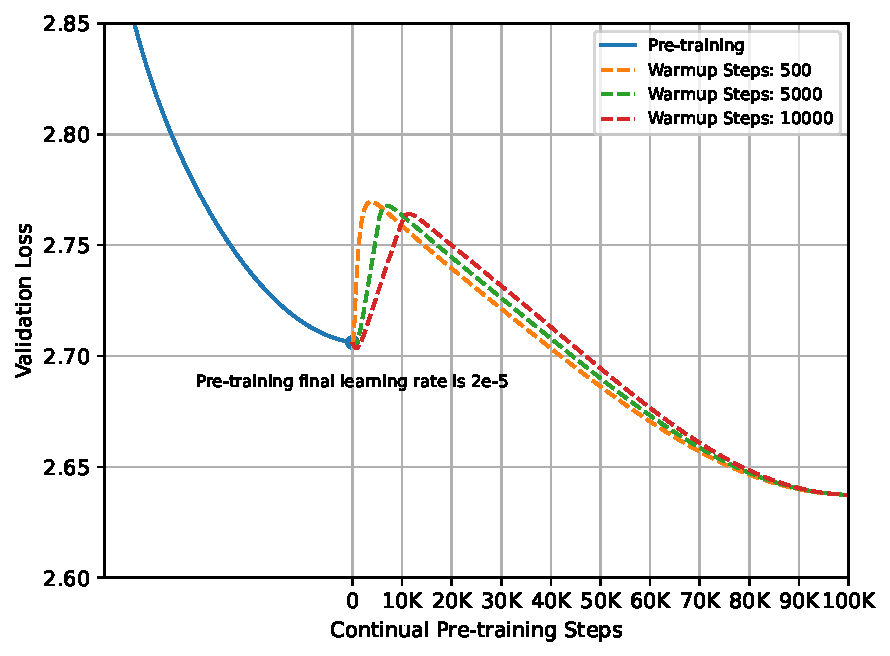
\includegraphics[width=\textwidth]{images/rewp-steps.pdf}
        \caption{The predicted validation loss with different re-warmup max learning rate in the continual pre-training process. }
        \label{fig:phe-match-cpt-step}
    \end{subfigure}
    \caption{The predicted validation loss with different re-warmup max learning rate and re-warmup steps in the continual pre-training process. The LRS of continual pre-training is cosine ($T$=100K) and the min learning rate is 0.}
\label{fig:phe-match:2}
\end{figure}